% \iffalse
\let\negmedspace\undefined
\let\negthickspace\undefined
\documentclass[journal,12pt,twocolumn]{IEEEtran}
\usepackage{float}
\usepackage{circuitikz}
\usepackage{cite}
\usepackage{amsmath,amssymb,amsfonts,amsthm}
\usepackage{algorithmic}
\usepackage{graphicx}
\usepackage{textcomp}
\usepackage{xcolor}
\usepackage{txfonts}
\usepackage{listings}
\usepackage{amsmath}
\usepackage{enumitem}
\usepackage{mathtools}
\usepackage{gensymb}
\usepackage{comment}
\usepackage[breaklinks=true]{hyperref}
\usepackage{tkz-euclide} 
\usepackage{listings}
\usepackage{gvv}                                        
\def\inputGnumericTable{}                                 
\usepackage[latin1]{inputenc}                                
\usepackage{color}                                            
\usepackage{array}                                            
\usepackage{longtable}                                       
\usepackage{calc}                                             
\usepackage{multirow}                                         
\usepackage{hhline}                                           
\usepackage{ifthen}                                           
\usepackage{lscape}
\newtheorem{theorem}{Theorem}[section]
\newtheorem{problem}{Problem}
\newtheorem{proposition}{Proposition}[section]
\newtheorem{lemma}{Lemma}[section]
\newtheorem{corollary}[theorem]{Corollary}
\newtheorem{example}{Example}[section]
\newtheorem{definition}[problem]{Definition}
\newcommand{\BEQA}{\begin{eqnarray}}
\newcommand{\EEQA}{\end{eqnarray}}
\newcommand{\define}{\stackrel{\triangle}{=}}
\theoremstyle{remark}
\newtheorem{rem}{Remark}
\begin{document}

\bibliographystyle{IEEEtran}
\vspace{3cm}
\title{Audio Filter}
\author{EE23BTECH11006 - Ameen Aazam$^{*}$% <-this % stops a space
}
\maketitle
\newpage
\bigskip
\renewcommand{\thefigure}{\arabic{figure}}
\renewcommand{\thetable}{\theenumi}

\bibliographystyle{IEEEtran}
\begin{enumerate}[label=\thesection.\arabic*
,ref=\thesection.\theenumi]
\section{Digital Filter}
\label{input_sound}
\item The sound file I have used in this audio filter project is available in this link
\begin{lstlisting}
https://github.com/Ameen-etc/Audio-Filter/blob/main/codes/Tomar_%20Khola_Hawa.wav
\end{lstlisting}
\item 
\label{Python code}
This is the Python code used for filtering the audio signal :
\lstinputlisting{codes/Noise_Reduction.py}
\item \label{Spectrum}
The mentioned audio file is analyzed with a spectrogram, using the open source platform \href{https://academo.org/demos/spectrum-analyzer}{\url{https://academo.org/demos/spectrum-analyzer}}.\\
Darker areas represent very low amplitude while the orange and yellow areas denote high intensity in the corresponding frequencies.
\begin{figure}[h!]
    \centering
    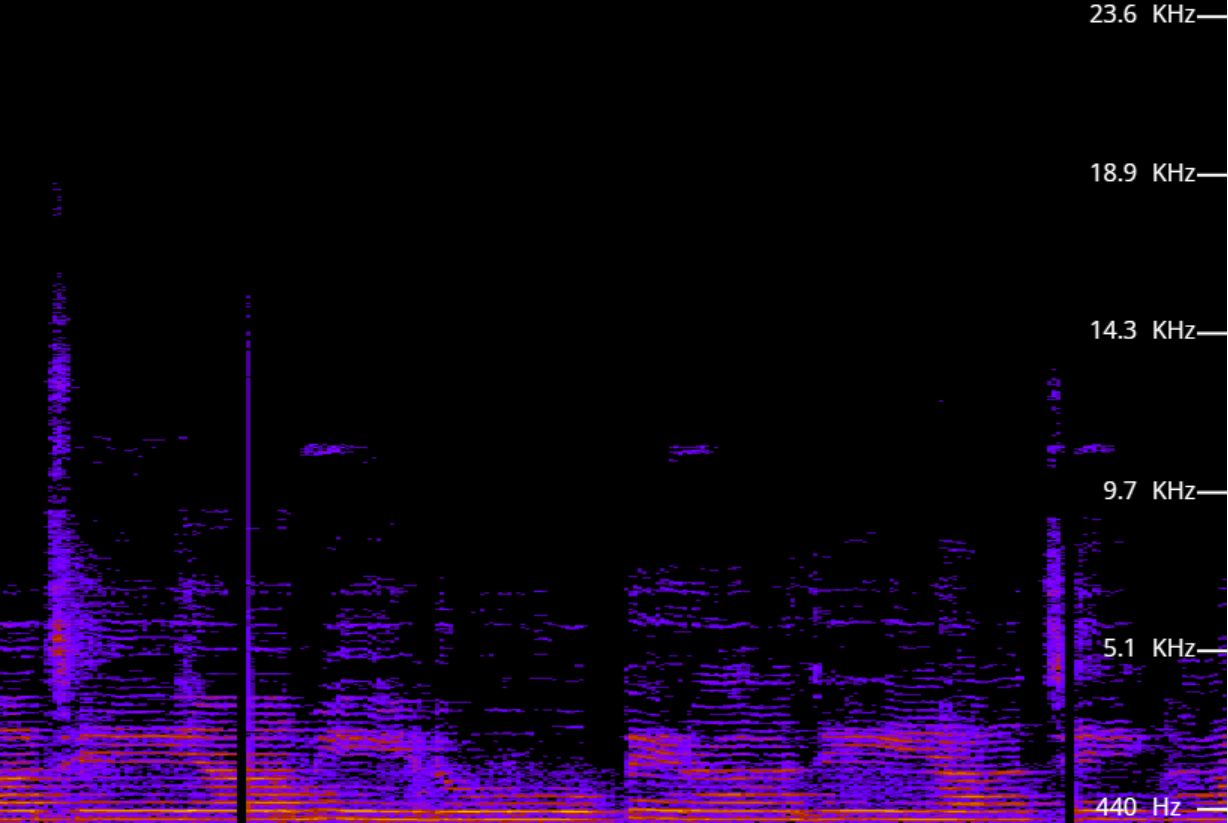
\includegraphics[width=0.7\columnwidth]{figs/test_sig.png}
    \caption{Raw Audio}
    \label{fig:raw_file}
\end{figure}
\newline
This is the spectrum of the original recorded audio.
\begin{figure}[h!]
    \centering
    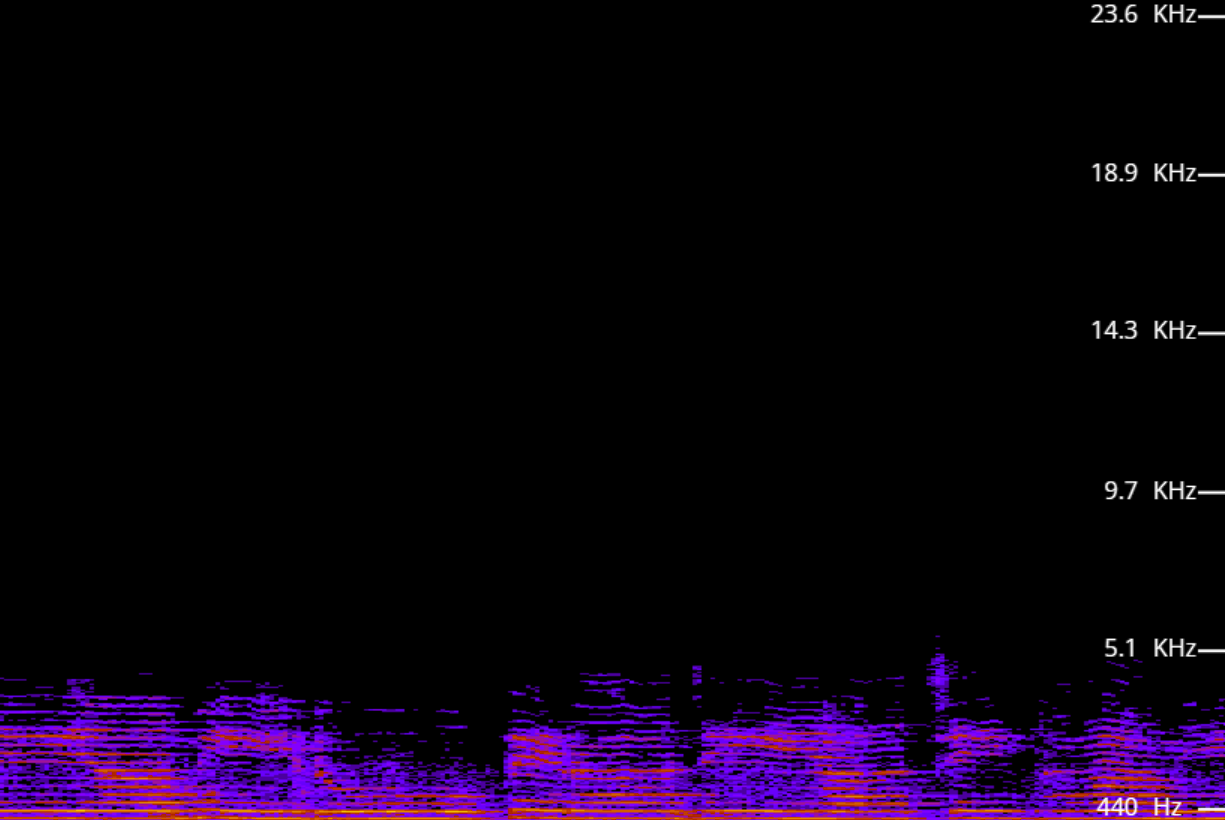
\includegraphics[width=0.7\columnwidth]{figs/out_sig.png}
    \caption{Filtered Audio}
    \label{fig:filtered_audio}
\end{figure}
\newline
And this is after the filtering. As we can see higher frequency components ($>4kHz$) in the original signal have been significantly diminished in the filtered output.
\end{enumerate}
\section{Difference Equation}
\begin{enumerate}[label=\thesection.\arabic*,ref=\thesection.\theenumi]
\item Let
\begin{equation}
x(n) = \cbrak{\underset{\uparrow}{1},2,3,4,2,1} \label{prob:2.1}
\end{equation}
Sketch $x(n)$. 
\item Let
\begin{multline}
y(n) + \frac{1}{2}y(n-1) = x(n) + x(n-2), 
\\
y(n) = 0, n < 0 \label{prob:2.2}
\end{multline}
Sketch $y(n)$.\\
Solve\\
The following C code calculates $y(n)$ and stores the data points in a dat file.
\begin{lstlisting}
    https://github.com/Ameen-etc/Audio-Filter/blob/main/codes/y.c
\end{lstlisting}
Now this python code uses the dat file to plot the stem plot of $y(n)$.
\begin{lstlisting}
    https://github.com/Ameen-etc/Audio-Filter/blob/main/codes/plot.py
\end{lstlisting}
And this is the obtained plot of $x(n)$ and $y(n)$,
\begin{figure}[h!]
    \centering
    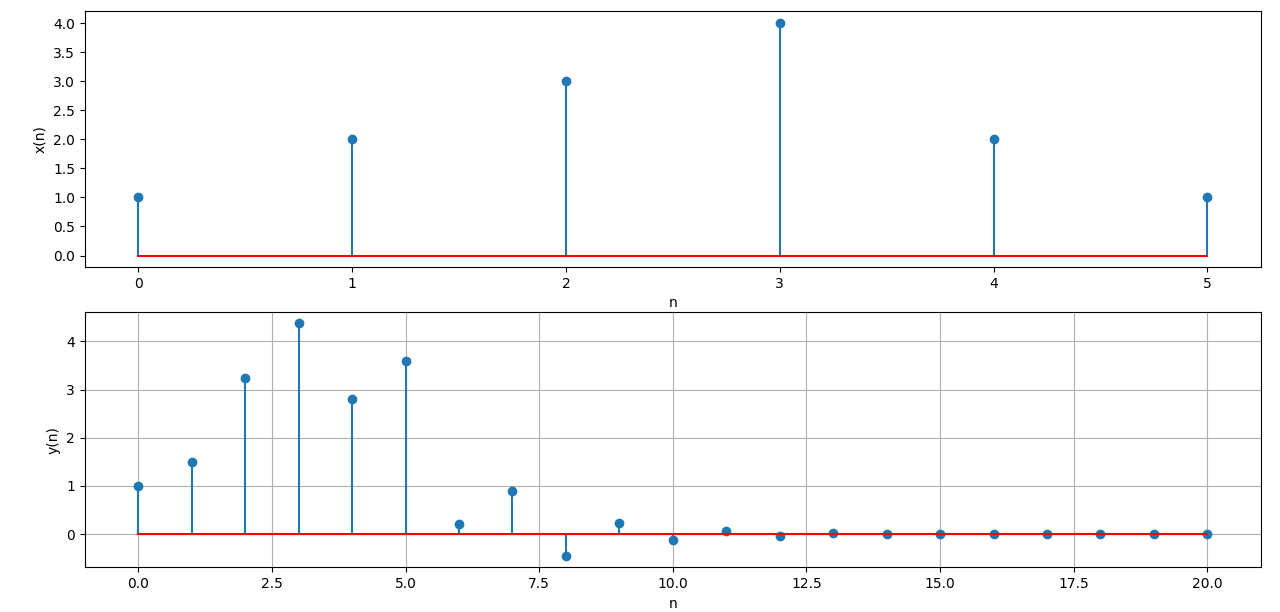
\includegraphics[width=\columnwidth]{figs/x and y.png}
    \caption{Plot of $x(n)$ and $y(n)$}
    \label{fig:x-y}
\end{figure}
\end{enumerate}
\section{Z-Transform}

\begin{enumerate}[label=\thesection.\arabic*]
\item The $Z$-transform of $x(n)$ is defined as
%
\begin{equation}
X(z)={\mathcal {Z}}\{x(n)\}=\sum _{n=-\infty }^{\infty }x(n)z^{-n} \label{eq:z_tf}
\end{equation}
%
Show that
\begin{equation}
{\mathcal {Z}}\{x(n-1)\} = z^{-1}X(z)\label{eq:1_shift}
\end{equation}
and find
\begin{equation}
	{\mathcal {Z}}\{x(n-k)\} 
\end{equation}
\solution From \eqref{eq:z_tf},
\begin{align}
{\mathcal {Z}}\{x(n-k)\} &=\sum _{n=-\infty }^{\infty }x(n-1)z^{-n}
\\
&=\sum _{n=-\infty }^{\infty }x(n)z^{-n-1} = z^{-1}\sum _{n=-\infty }^{\infty }x(n)z^{-n}
\end{align}
resulting in \eqref{eq:1_shift}. Similarly, it can be shown that
%
\begin{equation}
	{\mathcal {Z}}\{x(n-k)\} = z^{-k}X(z) \label{eq:k_shift}
\end{equation}
\item Find
%
\begin{equation}
H(z) = \frac{Y(z)}{X(z)}
\end{equation}
from  \eqref{prob:2.2} assuming that the $Z$-transform is a linear operation.
\\
\solution  Applying \eqref{eq:k_shift} in \eqref{prob:2.2},
\begin{align}
Y(z) + \frac{1}{2}z^{-1}Y(z) &= X(z)+z^{-2}X(z)
\\
\implies \frac{Y(z)}{X(z)} &= \frac{1 + z^{-2}}{1 + \frac{1}{2}z^{-1}}
\label{eq:transfer_fn}
\end{align}
%
\item Find the Z transform of 
\begin{equation}
\delta(n)
=
\begin{cases}
1 & n = 0
\\
0 & \text{otherwise}
\end{cases}
\end{equation}
and show that the $Z$-transform of
\begin{equation}
\label{eq:unit_step}
u(n)
=
\begin{cases}
1 & n \ge 0
\\
0 & \text{otherwise}
\end{cases}
\end{equation}
is
\begin{equation}
U(z) = \frac{1}{1-z^{-1}}, \quad \abs{z} > 1
\end{equation}
\solution It is easy to show that
\begin{equation}
\delta(n) \system{Z} 1
\end{equation}
and from \eqref{eq:unit_step},
\begin{align}
U(z) &= \sum _{n= 0}^{\infty}z^{-n}
\\
&=\frac{1}{1-z^{-1}}, \quad \abs{z} > 1
\end{align}
using the formula for the sum of an infinite geometric progression.
%
\item Show that 
\begin{equation}
\label{eq:anun}
a^nu(n) \system{Z} \frac{1}{1-az^{-1}} \quad \abs{z} > \abs{a}
\end{equation}
\solution 
\begin{align}
    a^nu(n) &\system{Z} \sum_{n=-\infty}^{+\infty}a^nu(n)z^{-n}\\
    &=\sum_{n=-\infty}^{0}a^nz^{-n} \\
    &=\frac{1}{1-az^{-1}} \quad \abs{z} > \abs{a}
\end{align}
%
\item 
Let
\begin{equation}
H\brak{e^{\j \omega}} = H\brak{z = e^{\j \omega}}.
\end{equation}
Plot $\abs{H\brak{e^{\j \omega}}}$.  Comment.  $H(e^{\j \omega})$ is
known as the {\em Discret Time Fourier Transform} (DTFT) of $h(n)$.
\\
\solution
Substituting $z=e^{j\omega}$ in \eqref{eq:transfer_fn} and taking the modulus, we get,
\begin{align}
    \left|H\brak{e^{j\omega}}\right|&=\left|\frac{1+e^{-2j\omega}}{1+\frac{1}{2}e^{-j\omega}}\right| \\
    \left|H\brak{e^{j\brak{\omega+2\pi}}}\right|&=\left|\frac{1+e^{-2j\brak{\omega+2\pi}}}{1+\frac{1}{2}e^{-j\brak{\omega+2\pi}}}\right| \\
    &=\left|\frac{1+e^{-2j\omega}\cdot e^{-4j\pi}}{1+\frac{1}{2}e^{-j\omega}\cdot e^{-2j\pi}}\right| \\
    &=\left|\frac{1+e^{-2j\omega}}{1+\frac{1}{2}e^{-j\omega}}\right|\\
    &=\left|H\brak{e^{j\omega}}\right|
\end{align}
So this verifies DTFT of any signal is always periodic with the fundamental period of $2\pi$.
Now the following Python code plots the magnitude of the transfer function.
\begin{lstlisting}
    https://github.com/Ameen-etc/Audio-Filter/blob/main/codes/3.5.py
\end{lstlisting}
And this is the plot,
\begin{figure}[h!]
    \centering
    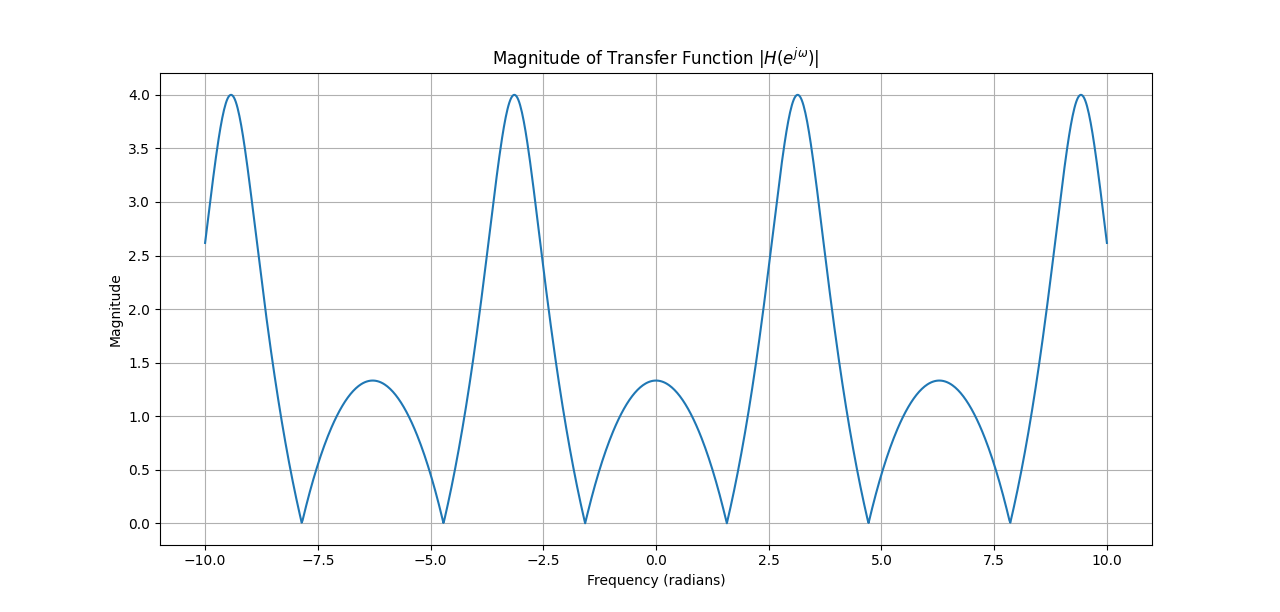
\includegraphics[width=\columnwidth]{figs/3.5.png}
    \caption{$\left|H\brak{e^{j\omega}}\right|$}
    \label{fig:tfm}
\end{figure}
\end{enumerate}
\section{Impulse Response}
\begin{enumerate}[label=\thesection.\arabic*]
\item \label{prob:impulse_resp}
Find an expression for $h(n)$ using $H(z)$, given that 
%in Problem \ref{eq:ztransab} and \eqref{eq:anun}, given that
\begin{equation}
\label{eq:impulse_resp}
h(n) \system{Z} H(z)
\end{equation}
and there is a one to one relationship between $h(n)$ and $H(z)$. $h(n)$ is known as the {\em impulse response} of the
system defined by \eqref{prob:2.2}.
\\
\solution From \eqref{eq:freq_resp},
\begin{align}
H(z) &= \frac{1}{1 + \frac{1}{2}z^{-1}} + \frac{ z^{-2}}{1 + \frac{1}{2}z^{-1}}
\\
\implies h(n) &= \brak{-\frac{1}{2}}^{n}u(n) + \brak{-\frac{1}{2}}^{n-2}u(n-2)
\end{align}
using \eqref{eq:anun} and \eqref{eq:k_shift}.
\item Sketch $h(n)$. Is it bounded? Convergent? 
\\
\solution The following code plots $h\brak{n}$ 
\begin{lstlisting}
https://github.com/Ameen-etc/Audio-Filter/blob/main/codes/4.2.py
\end{lstlisting}
\begin{figure}[h!]
    \centering
    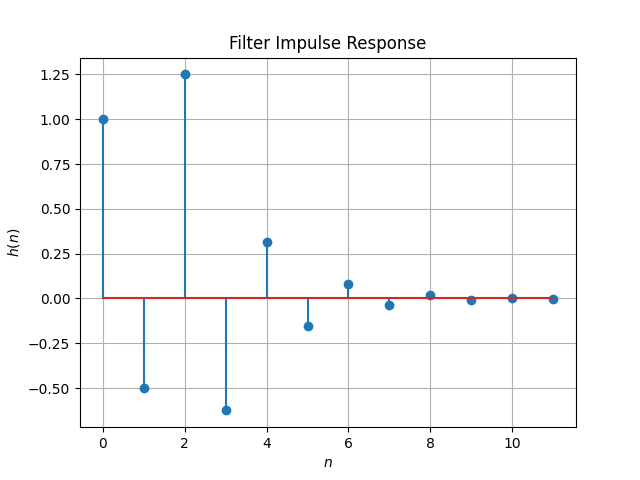
\includegraphics[width=\columnwidth]{figs/hn.png}
    \caption{$h(n)$ as the inverse of $H(z)$}
    \label{fig:hn}
\end{figure}
%
\item The system with $h(n)$ is defined to be stable if
\begin{equation}
\sum_{n=-\infty}^{\infty}h(n) < \infty \label{eq:stable}
\end{equation}
Is the system defined by \eqref{prob:2.2} stable for the impulse response in \eqref{eq:impulse_resp}?\\

The convergence of \eqref{eq:stable} is obtained by the tes,
\begin{align}
    \lim_{n \to \infty}\left|\frac{h\brak{n+1}}{h\brak{n}}\right|<1
\end{align}
Now for any $n>0$ $\delta\brak{n-2}=\delta\brak{n}=0$.
Now using this in \eqref{prob:2.2},
\begin{align}
    \lim_{n \to \infty}\left|\frac{h\brak{n+1}}{h\brak{n}}\right|=\frac{1}{2}<1
\end{align}
So the sum is converging and the system is stable.

\item 
Compute and sketch $h(n)$ using 
\begin{equation}
\label{eq:iir_filter_h}
h(n) + \frac{1}{2}h(n-1) = \delta(n) + \delta(n-2), 
\end{equation}
%
This is the definition of $h(n)$.
\\
\solution\\
Definition of $h\brak{n}$: The output of the system when $\delta\brak{n}$ is given as input.\\

The following code plots Fig. \ref{fig:hndef}. Note that this is the same as Fig. 
\ref{fig:hn}. 

\begin{lstlisting}
https://github.com/Ameen-etc/Audio-Filter/blob/main/codes/hndef.py
\end{lstlisting}
\begin{figure}[h!]
\centering
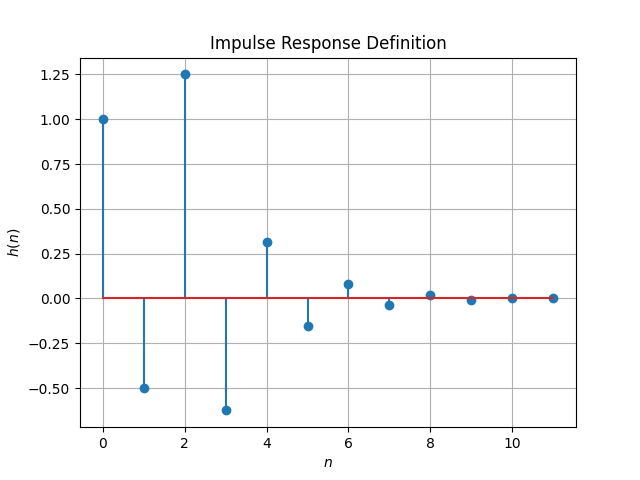
\includegraphics[width=\columnwidth]{figs/hndef}
\caption{$h(n)$ from the definition is same as \figref{fig:hn}}
\label{fig:hndef}
\end{figure}
\item Compute 
%
\begin{equation}
\label{eq:convolution}
y(n) = x(n)*h(n) = \sum_{n=-\infty}^{\infty}x(k)h(n-k)
\end{equation}
%
Comment. The operation in \eqref{eq:convolution} is known as
{\em convolution}.
%
\\
\solution The following code plots Fig. \ref{fig:ynconv}. Note that this is the same as $y(n)$ in  Fig. \ref{fig:x-y}. 
%
\begin{lstlisting}
https://github.com/Ameen-etc/Audio-Filter/blob/main/codes/4.5.py
\end{lstlisting}
\begin{figure}[H]
\centering
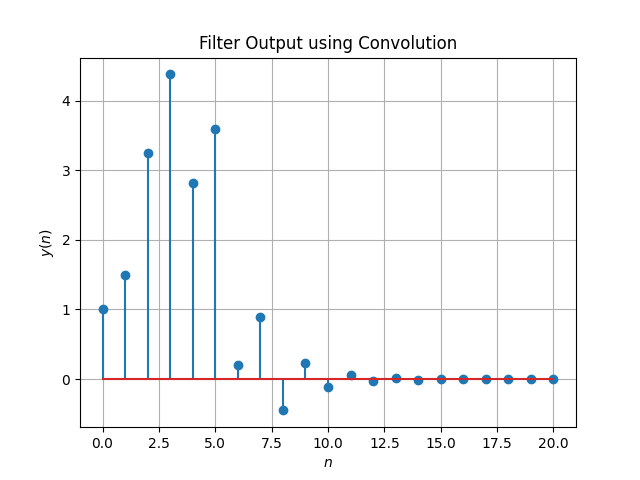
\includegraphics[width=\columnwidth]{figs/ynconv.png}
\caption{$y(n)$ from the definition of convolution}
\label{fig:ynconv}
\end{figure}
\item Show that
\begin{equation}
y(n) =  \sum_{n=-\infty}^{\infty}x(n-k)h(k)
\end{equation}
\solution
In \eqref{eq:convolution}, if we substitute $k = n - k$,
\begin{align}
y\brak{n} &= \sum_{k=-\infty}^{\infty}x\brak{k}h\brak{n - k} \\
		  &= \sum_{n - k=-\infty}^{\infty}x\brak{n - k}h\brak{k} \\
		  &= \sum_{k=-\infty}^{\infty}x\brak{n - k}h\brak{k}
\end{align}
\end{enumerate}
\section{DFT and FFT}
\begin{enumerate}[label=\thesection.\arabic*]
\item
Compute
\begin{equation}
X(k) \define \sum _{n=0}^{N-1}x(n) e^{-\j2\pi kn/N}, \quad k = 0,1,\dots, N-1
\end{equation}
and $H(k)$ using $h(n)$.
\item Compute 
\begin{equation}
Y(k) = X(k)H(k)
\label{eq:fp}
\end{equation}
\item Compute
\begin{equation}
y\brak{n}={\frac {1}{N}}\sum _{k=0}^{N-1}Y\brak{k}\cdot e^{\j 2\pi kn/N},\quad n = 0,1,\dots, N-1
\label{eq:inv-ft}
\end{equation}

\solution The following code solves the above problems and plots the following output using DFT.
\begin{lstlisting}
    https://github.com/Ameen-etc/Audio-Filter/blob/main/codes/6.py
\end{lstlisting}
\begin{figure}[h!]
    \centering
    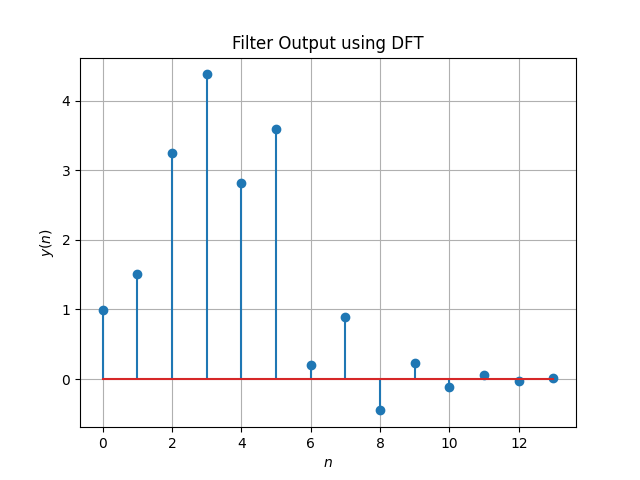
\includegraphics[width=\columnwidth]{figs/6-dft.png}
    \caption{$y\brak{n}$ from DFT}
    \label{fig:enter-label}
\end{figure}
\vspace{1cm}
\item Repeat the previous exercise by computing $X(k), H(k)$ and $y(n)$ through FFT and IFFT.
\solution The following code uses FFT and IFFT for solving the previous question,
\begin{lstlisting}
    https://github.com/Ameen-etc/Audio-Filter/blob/main/codes/5.4.py
\end{lstlisting}
And this is plot $y(n)$ obtained,
\begin{figure}[h!]
    \centering
    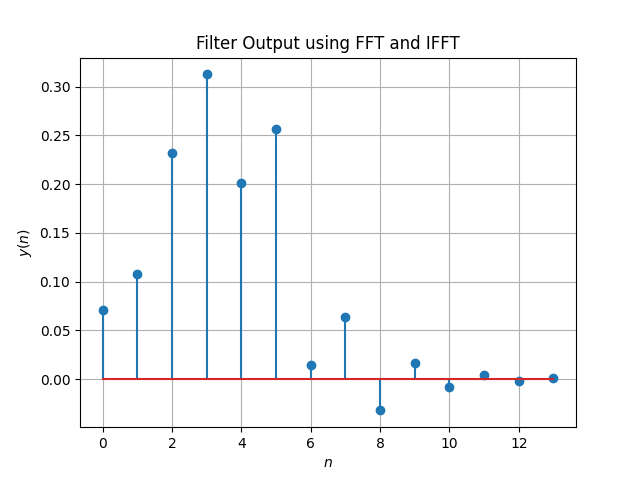
\includegraphics[width=\columnwidth]{figs/FFT and IFFT.png}
    \caption{$y(n)$ with FFT and IFFT}
\end{figure}
which matches our gained $y(n)$.
\vspace{1cm}
\item Wherever possible, express all the above equations as matrix equations.\\
\solution
The general expression for DFT is given as,
\begin{align}
    X\brak{k}&=\sum_{n=0}^{N-1}x\brak{n}e^{\frac{2\pi k}{N}n}
\end{align}
Here $N$ is number of samples of the original signal.
Now this equation can be expressed as a matrix equation as following,
\begin{align}
    \mathbf{X}=\mathbf{x}\mathbf{W}
\end{align}
Where $\mathbf{x}$ is the sample points, given as,
\begin{align}
    \mathbf{x}=\begin{pmatrix}
    x\brak{0} & x\brak{1} & x\brak{2} & \ldots & x\brak{N-1}
    \end{pmatrix}
\end{align}
And $\mathbf{W}$ is the DFT matrix, defined as,
\begin{align}
    \mathbf{W}=\begin{pmatrix}
        w^0 & w^0 & w^0 & \ldots & w^0 \\
        w^0 & w^1 & w^2 & \ldots & w^{N-1} \\
        w^0 & w^2 & w^4 & \ldots & w^{2(N-1)} \\
        \vdots & \vdots & \vdots & \ddots & \vdots \\
        w^0 & w^{N-1} & w^{2(N-1)} & \ldots & w^{(N-1)(N-1)}\\
    \end{pmatrix}
\end{align}
And the $\mathbf{X}$ matrix is the output matrix defined as,
\begin{align}
    \mathbf{X}=\begin{pmatrix}
    X\brak{0} & X\brak{1} & X\brak{2} & \ldots & X\brak{N-1}
    \end{pmatrix}
\end{align}
So we can express \eqref{eq:fp} as a matrix equation,
\begin{align}
	\mathbf{Y} &= \mathbf{X}\odot\mathbf{H} \\
        &= \brak{\mathbf{x}\mathbf{W}}\odot\brak{\mathbf{h}\mathbf{W}}
\end{align}
where the $\odot$ represents the Hadamard product which performs element-wise multiplication.
The following code provides the plot for $y(n)$ using the DFT matrix at first and then calculating IFFT,
\begin{lstlisting}
    https://github.com/Ameen-etc/Audio-Filter/blob/main/codes/5.5.py
\end{lstlisting}
\begin{figure}[h!]
    \centering
    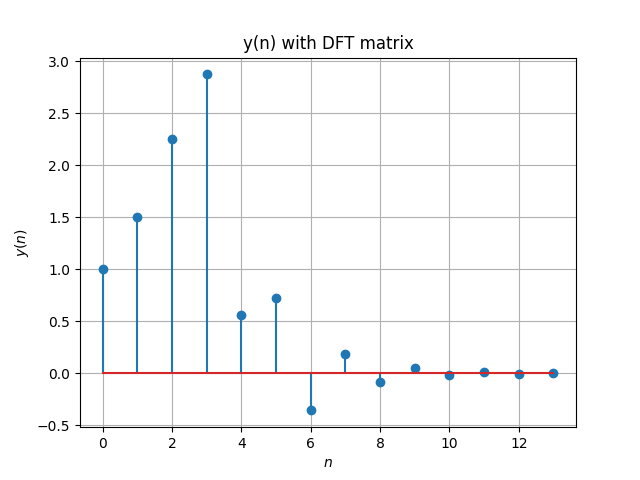
\includegraphics[width=\columnwidth]{figs/dft.png}
    \caption{$y(n)$ with DFT matrix}
    \label{fig:DFTMT}
\end{figure}
\end{enumerate}
\section{\underline{EXERCISES}}
\noindent Answer the following questions by looking at the python code in Problem \ref{Python code}.


\begin{enumerate}[label=\thesection.\arabic*]
\vspace{1cm}
\item The command
\begin{lstlisting}
	output_signal = signal.lfilter(b, a, input_signal)
	\end{lstlisting}
in Problem \ref{Python code} is executed through the following difference equation
\begin{equation}
\label{eq:iir_filter_gen}
 \sum _{m=0}^{M}a\brak{m}y\brak{n-m}=\sum _{k=0}^{N}b\brak{k}x\brak{n-k} 
\end{equation}
%
where the input signal is $x(n)$ and the output signal is $y(n)$ with initial values all 0. Replace
\textbf{signal. filtfilt} with your own routine and verify.\\
\solution
The following code gives the filtered output of the audio signal we are using, without using the inbuilt function.
\begin{lstlisting}
    https://github.com/Ameen-etc/Audio-Filter/blob/main/codes/6.1.py
\end{lstlisting}
And this is the plot we will be getting,
\begin{figure}[h!]
    \centering
    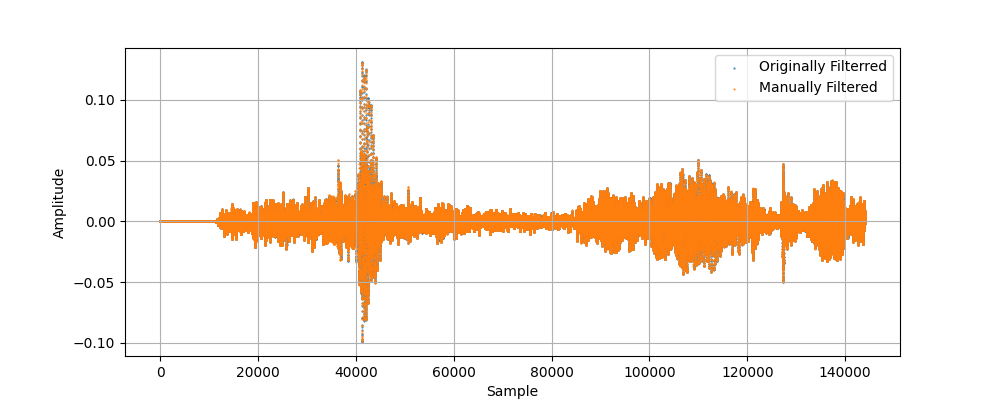
\includegraphics[width=\columnwidth]{figs/manualvsfun.png}
    \caption{Originally filtered $vs.$ Manually filtered}
    \label{fig:enter-label}
\end{figure}
And as we can see, our output matches with the previously filtered output.
\vspace{1cm}
\item Repeat all the exercises in the previous sections for the above $a$ and $b$.\\
\solution The values of $a$ and $b$, we can get from the above code itself and those can be used to form the difference equation.
As a $4^{th}$ order Butterworth filter we will be having,
\begin{align}
    M&=4\\
    N&=4
\end{align}
And we will be getting the difference equation like,
\begin{align}
\begin{split}
    &a(0)y(n)+a(1)y(n-1)+a(2)y(n-2)+\\
    &a(3)y(n-3)+a(4)y(n-4)=b(0)x(n)+\\
    &b(1)x(n-1)+b(2)x(n-2)+b(3)x(n-3)\\
    &+b(4)x(n-4) \label{eq:diff}
\end{split}
\end{align}
Now, using the values of $a$s and $b$s we will have,
\begin{align}
    \begin{split}
        &y(n)-2.64y(n-1)+2.77y(n-2)-\\
    &1.34y(n-3)+0.25y(n-4)=0.003x(n)+\\
    &0.010x(n-1)+0.015x(n-2)+0.010x(n-3)\\
    &+0.003x(n-4)
    \end{split}
\end{align}
So from \eqref{eq:diff} we can have the transfer function as,
\begin{align}
    H(z)=\frac{b(0)+b(1)z^{-1}+b(2)z^{-1}+b(3)z^{-3}+b(4)z^{-4}}{a(0)+a(1)z^{-1}+a(2)z^{-1}+a(3)z^{-3}+a(4)z^{-4}}
\end{align}
And we can split it into partial fractions,
\begin{align}
    H(z)=\sum_{i=1}^{4}\brak{\frac{P_i}{1-Q_iz^{-1}}}+R
\end{align}
And then using inverse Z-transform,
\begin{align}
h(n) &= \sum_{i=1}^{4}\sbrak{P_iQ^n_iu(n)} + R\delta(n)
	\label{eq:h-n-expr}
\end{align}
This code is used to get the corresponding g values of $P$, $Q$, and $R$,
\begin{lstlisting}
    https://github.com/Ameen-etc/Audio-Filter/blob/main/codes/residue.py
\end{lstlisting}
And the values are listed below,
\begin{table}[H]
    \centering
    \renewcommand\thetable{1}
    \setlength{\extrarowheight}{9pt}
    \resizebox{0.51\textwidth}{!}{
    \begin{tabular}{|c|c|c|}
    \hline
    \textbf{$P_i$} & \textbf{$Q_i$} & \textbf{$R$} \\ \hline
    $0.21814719-0.35050232j$ &$0.592381+0.13088214j$&$0.00257643$  \\ \hline
    $0.21814719+0.35050232j$ &$0.592381-0.13088214j$&$-$  \\ \hline
    $-0.2095952-0.0102857j$ &$0.72693287+0.3877475j$&$-$  \\ \hline
    $-0.2095952+0.0102857j$ &$0.72693287-0.3877475j$&$-$  \\ \hline
    \end{tabular}}
    \caption{Residue Values}
    \label{tab:Residue Values}
    \end{table}

\begin{itemize}
\vspace{1cm}
    \item {Stability of $h(n)$}:\\
$h(n)$ will be stable if it's Z-transform contains the unit circle or $H(z)$ is defined for $z=1$
\begin{align}
H\brak{z} &= \sum_{n = 0}^{\infty} h\brak{n}z^{-n}\\
H(1)&= \sum_{n = 0}^{\infty}h(n)  = \frac{\sum_{k = 0}^{4}b(k)}{\sum_{k = 4}^{M}a(k)}< \infty
\end{align}
As all $a(k)$ s and $b(k)$ s are finite, the sum converges. And hence, the impulse response is stable.
\end{itemize}
Now this code provides the following discrete-time Butterworth filter frequency response,
\begin{lstlisting}
    https://github.com/Ameen-etc/Audio-Filter/blob/main/codes/discrete-time-res.py
\end{lstlisting}
\begin{figure}[h!]
    \centering
    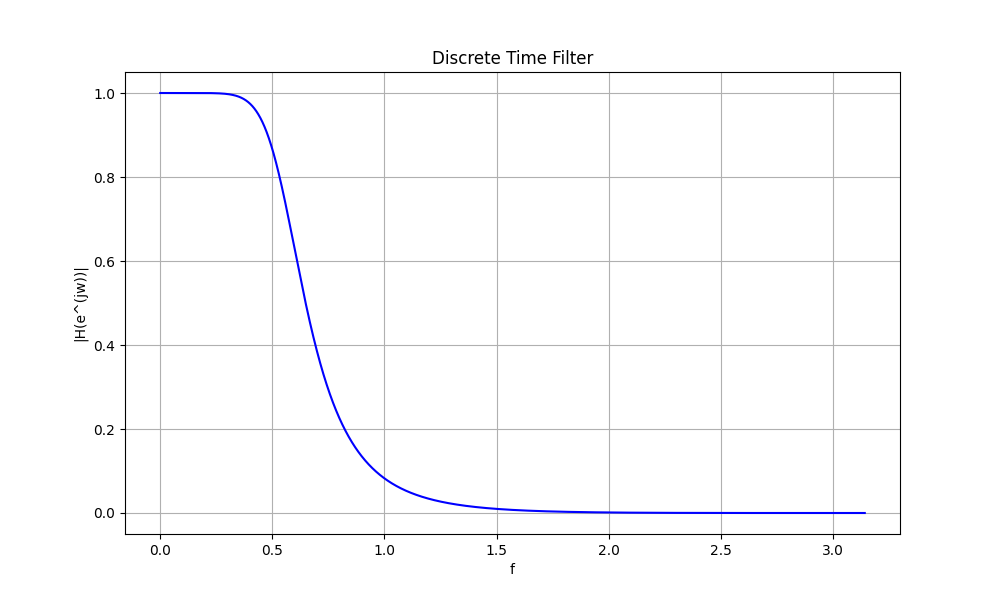
\includegraphics[width=\columnwidth]{figs/discrete-res.png}
    \caption{Discrete-time response}
\end{figure}
Now using Bilinear Transform by replacing 
\begin{align}
    z=\frac{1-\frac{T}{2}s}{1+\frac{T}{2}s}
\end{align}
we will be getting the continuous-time analog response. And the following code does that,
\begin{lstlisting}
    https://github.com/Ameen-etc/Audio-Filter/blob/main/codes/analog-res.py
\end{lstlisting}
And this is the obtained frequency response,
\begin{figure}[h!]
    \centering
    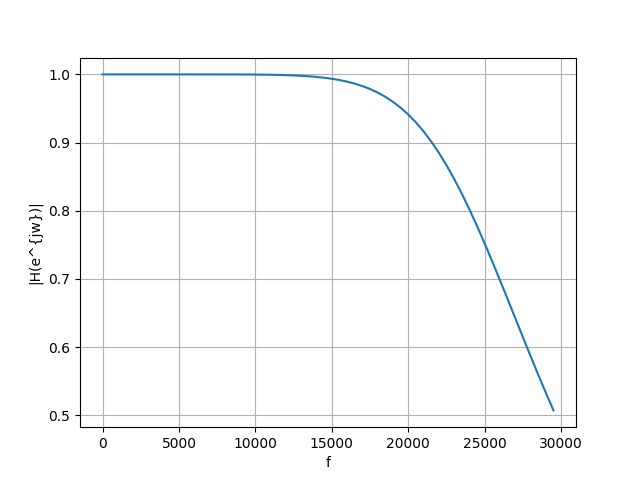
\includegraphics[width=\columnwidth]{figs/analog.png}
    \caption{Continuous-time response}
\end{figure}
Now this code plots the pole-zero plot of the filter,
\begin{lstlisting}
    https://github.com/Ameen-etc/Audio-Filter/blob/main/codes/pole-zero.py
\end{lstlisting}
\begin{figure}[h!]
    \centering
    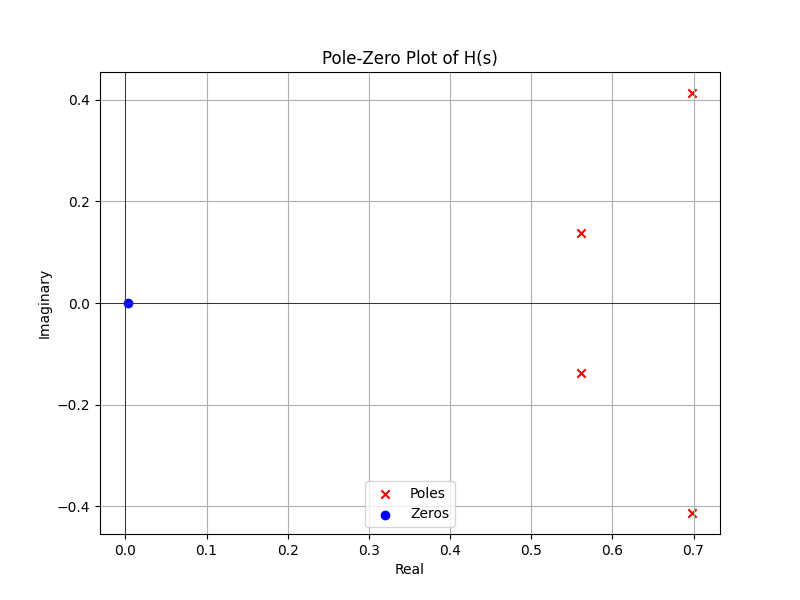
\includegraphics[width=\columnwidth]{figs/x-0.png}
    \caption{Pole-Zero Plot}
\end{figure}
\vspace{1cm}
\item Implement your own fft routine in C and call this fft in python.\\

The following C code calculates the fft of any predefined array manually,
\begin{lstlisting}
    https://github.com/Ameen-etc/Audio-Filter/blob/main/codes/fft.c
\end{lstlisting}
Now, to call this C function in the python code, we have to create a shared library by using the bash script,
\begin{lstlisting}
    gcc -shared -o fft.dll -fPIC fft.c
\end{lstlisting}
And this is the python code which calls the C function to perform fft,
\begin{lstlisting}
    https://github.com/Ameen-etc/Audio-Filter/blob/main/codes/fft.py
\end{lstlisting}
\vspace{1cm}
\item Find the time complexities of computing y(n)
using FFT/IFFT and convolution and Compare.\\
The below code plots the time taken for the calculation of $y(n)$ using convolution against FFT/IFFT method,
\begin{lstlisting}
    https://github.com/Ameen-etc/Audio-Filter/blob/main/codes/timecom.py
\end{lstlisting}
And this is the result,
\begin{figure}[h!]
    \centering
    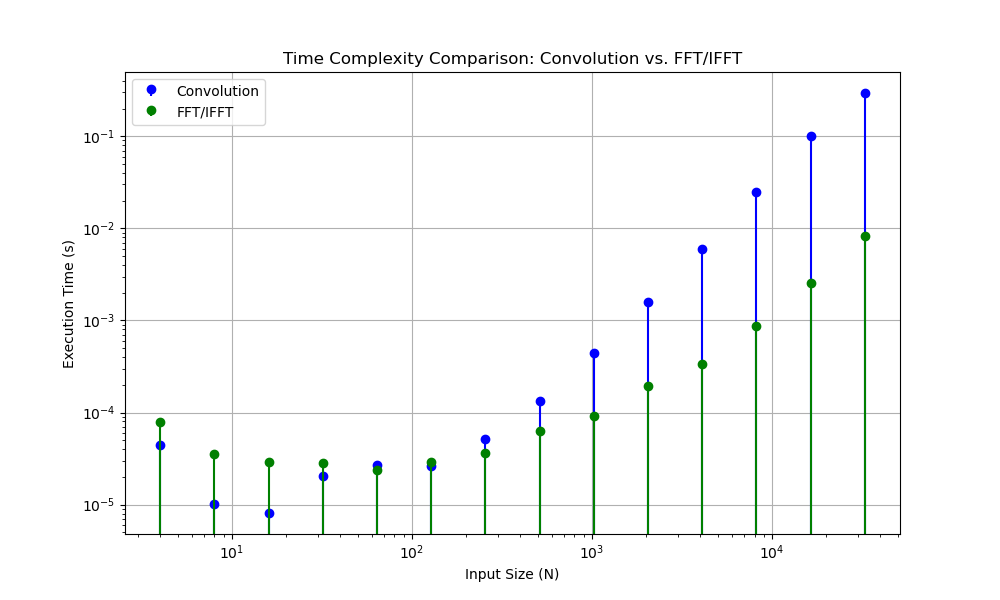
\includegraphics[width=\columnwidth]{figs/timecom.png}
    \caption{Time Complexity}
    \label{fig:enter-label}
\end{figure}
\item What is the sampling frequency of the input signal?\\
\solution The Sampling Frequency is 44.1KHz
\item
What is type, order and  cutoff-frequency of the above butterworth filter
\\
\solution The given butterworth filter is lowpass with order=4 and cutoff-frequency=1kHz.

\item
Modify the code with different input parameters and get the best possible output.

\solution
A better filtering can be found by setting the order of the filter higher.
\end{enumerate}
\end{document}
